\lecture{Introduction}{13:00}{26/09/23}{Tamer Elboghdadly}

\section*{Operating Systems}

\begin{itemize}
  \item The Operating System sits inbetween the hardware and application software
  \item It usually is not the actual GUI, but provides functionality for the applications which implement it
  \item OSes typically provide abstractions for applications so that they can run on different hardware
\end{itemize}

\subsection*{User and Kernel Mode}

\begin{itemize}
  \item User mode
  \begin{itemize}
    \item The programs that a user directly interacts with
    \item Uses an API to access hardware, rather than having direct access
  \end{itemize}
  \item Kernel mode
  \begin{itemize}
    \item The programs that run the operating system
    \item Has direct access to hardware
  \end{itemize}
\end{itemize}

\subsection*{System and Application Software}

\begin{itemize}
  \item Application software
  \begin{itemize}
    \item Programs that allow a user to perform a task
    \item Requires the support of system software to run
  \end{itemize}
  \item System software
  \begin{itemize}
    \item Software directly related to the operating system
    \item Manages the boot process
    \item Hardware drivers
    \item File system management
  \end{itemize}
\end{itemize}

\subsection*{The main functions of an Operating System}

\begin{itemize}
  \item Resource management
  \begin{itemize}
    \item Manages the memory, CPU and other hardware to allow multiple programs to run concurrently
    \item Handles requests from applications to allocate more resources
  \end{itemize}
  \item "Extended machine"
  \begin{itemize}
    \item Handles reading and writing to control registers, handlling interrupts, etc
    \item Provides higher level APIs for other software to interact with the hardware
  \end{itemize}
\end{itemize}

\section*{CPU Organisation}

\subsection*{Registers}

\begin{figure}[h]
  \centering
  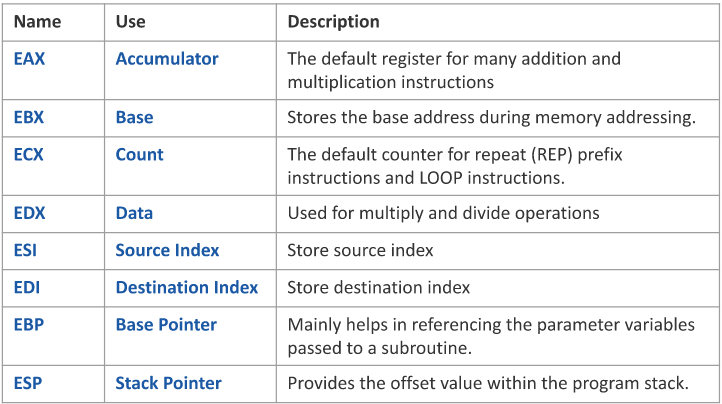
\includegraphics[width=0.8\textwidth]{registers.png}
  \caption{General purpose registers in an x86 Intel CPU}
\end{figure}

\begin{itemize}
  \item There are also special purpose registers, such as the Program Counter (PC) and the Program Status Word
  \item The Program Status Word sets the mode in which the CPU is operating
\end{itemize}

\subsection*{Assembly Language}

\begin{itemize}
  \item Assembly Language is the lowest-level programming language before Machine Code. It is slightly abstracted from machine code and uses neumonic symbols to represent instructions
  \item For example:
  \begin{itemize}
    \item \begin{verbatim}MOV EBX, EAX\end{verbatim}
    \item This copies the value in EAX into the EBX register
    \item \begin{verbatim}ADD EBX, 4\end{verbatim}
    \item This adds the value 4 to the EBX register
    \item This is equivalent to $b = a + 4$
  \end{itemize}
  \item The MOV instruction can also be used to move values between registers and the main memory
  \item I/O devices such as hard disks have a set of ports, which can be accessed to control the device and transfer data
  \item The special instructions IN and OUT are used to read from or write to ports
  \item For example:
  \begin{itemize}
    \item \begin{verbatim}IN EAX, 368\end{verbatim}
    \item This copies the value from the port 368 into the EAX register
  \end{itemize}
  \item The IN and OUT instructions can only be used when the CPU is running in Kernel Mode
\end{itemize}

\section*{User and Kernel Mode}

\begin{itemize}
  \item CPUs support running in two different modes: Kernel mode and User mode
  \item When running in User mode, some instructions (such as IN and OUT) cannot be used
  \item Typically, the Kernel of an operating system will run mostly or entirely in Kernel Mode
\end{itemize}

\section*{Interrupts}

\begin{itemize}
  \item When an external device needs to gain the attention of the CPU, it sends an interrupt
  \item A couple of examples are as follows
  \begin{itemize}
    \item When a disk has requested data in it's buffer
    \item When the key on an old PS/2 keyboard is pressed
  \end{itemize}
  \item When the CPU recieves an interrupt, it must abandon whatever it is currently doing and run an Interrupt Handler routine
  \item Interrupt Handlers run in Kernel mode
  \item The CPU places whatever resources it was using onto the stack and executes the interrupt handler. Once the handler has finished, it returns to the execution path stored on the stack
\end{itemize}